%%%%%%%%%%%%%%%%%%%%%%%%%%%%%%%%%%%%%%%%%%%%%%%%%%%%%%%%%%%%%%%%%%%%%%%%%%%%%%%%
%2345678901234567890123456789012345678901234567890123456789012345678901234567890
%        1         2         3         4         5         6         7         8

\documentclass[letterpaper, 10 pt, conference]{ieeeconf}  % Comment this line out if you need a4paper

%\documentclass[a4paper, 10pt, conference]{ieeeconf}      % Use this line for a4 paper

\IEEEoverridecommandlockouts                              % This command is only needed if 
                                                          % you want to use the \thanks command

\overrideIEEEmargins                                      % Needed to meet printer requirements.

% See the \addtolength command later in the file to balance the column lengths
% on the last page of the document

%\usepackage{graphics} % for pdf, bitmapped graphics files
% The following packages can be found on http:\\www.ctan.org
\usepackage{epsfig} % for postscript graphics files
\usepackage{mathptmx} % assumes new font selection scheme installed
\usepackage{times} % assumes new font selection scheme installed
\usepackage{amsmath} % assumes amsmath package installed
\usepackage{amssymb}  % assumes amsmath package installed
\usepackage{graphicx}
\usepackage{latexsym}
%\usepackage{amsthm}
\usepackage{fancyhdr}
%\usepackage{algorithmic}
\usepackage{cite}
\usepackage{array}
\usepackage{enumerate}

\newcommand{\argmin}{\arg\!\min}

\title{\LARGE \bf
Multi-View Object Recognition Using Hidden Markov Model and Relative Positioning}

%\title{\LARGE \bf
%An Odometry-Based Reinforcement Approach for Indoor Objects and Viewpoint Recognition
%}


\author{Luigi F. Tedesco$^{1}$, C\'eline Craye$^{2}$, Jean-Fran\c{c}ois Goudou$^{2}$ and David Filliat$^{1}$% <-this % stops a space
%\thanks{*This work was not supported by any organization}% <-this % stops a space
\thanks{$^{1}$U2IS, ENSTA ParisTech, Inria FLOWERS team, Universit\'e Paris-Saclay, 828 bd des Mar\'echaux, 91762 Palaiseau cedex France
{\tt\small tedesco@ensta.fr}}%
\thanks{$^{2}$Thales - SIX - Theresis - VisionLab 
1, avenue Augustin Fresnel, 91767 Palaiseau, France
{\tt\small celine.craye@thalesgroup.com}}%
}

%\author{Luigi F. Tedesco$^{1}$, C\'eline Craye$^{1}$, Jean-Fran\c{c}ois Goudou$^{2}$ and David Filliat$^{1}$% <-this % stops a space
%\thanks{*This work was not supported by any organization}% <-this % stops a space

%\thanks{$^{1}$U2IS, ENSTA ParisTech, Inria FLOWERS team, Universit\'e Paris-Saclay, 828 bd des Mar\'echaux, 91762 Palaiseau cedex France
%{\tt\small tedesco@ensta.fr}}
%\thanks{$^{2}$Thales - SIX - Theresis - VisionLab 
%1, avenue Augustin Fresnel, 91767 Palaiseau, France
%{\tt\small celine.craye@thalesgroup.com}}
%}
%\thanks{$^{1}$Luigi Franco Tedesco is a Master Student with Faculty of Electrical Engineering, Robotics and Artificial Intelligence,
        %ENSTA ParisTech, 91762 Palaiseau, France
        %{\tt\small tedesco@ensta.fr}}%
%\thanks{$^{2}$C\'eline Craye is a Doctoral Student with Faculty of Visual Saliency, Computer Vision and Developmental Robotics,
        %ENSTA ParisTech, 91762 Palaiseau, France
        %{\tt\small celine.craye@ensta-paristech.fr  }}%
%\thanks{$^{3}$Jean-Fran\c{c}ois Goudou is the R\&I Project Manager at the VisionLab, ThereSiS,
         %Thales Service, 91767 Palaiseau, France
        %{\tt\small jean-francois.goudou@thalesgroup.com}}%
%\thanks{$^{4}$David Filliat is with the Computer Science and System Ingeneering Laboratory,
        %ENSTA ParisTech, 91762 Palaiseau, France
        %{\tt\small david.filliat@ensta-paristech.fr }}%
%}

\begin{document}

\maketitle
\thispagestyle{empty}
\pagestyle{empty}


%%%%%%%%%%%%%%%%%%%%%%%%%%%%%%%%%%%%%%%%%%%%%%%%%%%%%%%%%%%%%%%%%%%%%%%%%%%%%%%%
\begin{abstract}

Object recognition capability is an essential condition for giving autonomy to mobiles robots in human designed environment. However, achieving this goal by relying only on a visual representation of the objects is a hard task. Fusing several sources of information to enhance representation can therefore be drastically helpful. In the context of object recognition in indoor environments, we present in this paper a procedure to integrate the odometric data in the classification process. When fused with visual perception, odometry incorporate the notion of diplacement between views that is able to overcome ambiguous points of view and associated misclassification. By observing objects from different perspectives and modeling the visual sequence as a Markovian process whose transitions are provided by odometry, our algorithm is able to copes with a sparse database, blurred images from motion and object spatial symmetry, to efficiently recognize objects and estimate the sequence of viewpoint at which they were observed. A multi-modal Kalman-based object tracking was also implemented in order to recognize multiple objects simultaneously. The approach was tested on a mobile robot and then compared with odometry-less recognition. The significant gap between the two approaches is very promising and reinforces the proposal of blending odometry and recognition. 

\end{abstract}


%%%%%%%%%%%%%%%%%%%%%%%%%%%%%%%%%%%%%%%%%%%%%%%%%%%%%%%%%%%%%%%%%%%%%%%%%%%%%%%%
\section{INTRODUCTION}

Object recognition for mobile robots in indoor cluttered environment is still an open problem. Recent progresses in computer vision techniques - typically deep learning based - have shown impressive results on complex image datasets \cite{krizhevsky2012imagenet}. However, those approach require heavy computation, large training datasets, and the recognition is based on RGB still images. On the other hand, mobile robots have the ability to move in their environment in order to modify and possibly improve their perception and representation. Relying on images without considering the displacement information is then a significant loss of information.

Objects and object-viewpoint recognition are among the most popular topics in robotics applications. Either used for environment exploration \cite{kragic2009object, ali2014contextual}, semantic navigation \cite{caron2014neural} or pose estimation for grasping \cite{bjorkman2004combination}, most of them typically rely on single-frame based recognition. Odometric information is also largely used on mobile robots in the context of object recognition, especially for the task of path planning \cite{roy2000isolated,meger2008curious}, tracking \cite{wang2007simultaneous} or simultaneous localization and mapping (SLAM) \cite{kragic2009object}. Although odometry is widely used to localize and track the position of objects, it is rarely used in the process of recognizing them. 

The use of RGB-D sensors in indoor environment has become very common because of their valuable information about the environment geometry. For this type of sensors, the object recognition pipeline is usually composed with a segmentation step followed by feature extraction before recognition itself. The segmentation step aims to differentiate objects from the background of raw images. By making the hypothesis that objects are represented in the scene as clusters of points right above a main plan, approaches such as \textit{Tabletop object detector} \cite{tabletop} and Caron et al. \cite{caron2014neural} determine the image main plane and search for objects clusters on top of it. Feature extraction is either RGB-based or geometrical. Among RGB features, bag of words of SIFTs or color histograms are commonly used \cite{csurka2004visual}. Deep features \cite{zhou2014learning} have also received a lot of attention recently, but their high dimensionality requires high computation performance to be processed in real time. Geometrical features based on point clouds are either local descriptor, such as SHOT \cite{tombari2010unique}, semi-global such as CVFH \cite{aldoma2012our}, or global \cite{rusu2009fast, rusu2010fast}.


Ambiguous viewpoints can easily trick single-view recognition approaches. Yet, considering the observation of objects as a sequence of distinctive but known points of view seems to be a natural way to deal with the problem. In that regard, a review of multi-view object representation can be found in \cite{roy2004active}. Among them, a solution inspired by human behavior for learning new unseen objects has been proposed by \cite{bulthoff2002view}, using key-frames and the rate of matching features with past frames, to overcome ambiguity in facial recognition task. Other approaches also use 3D CAD models \cite{aldoma2011cad} and graphs \cite{chakravarty1982characteristic} to enhance the internal representation of objects. Last, active approach aim to drive the robot displacement to improve its perception and reinforce the recognition capability of the robot, either based on reinforcement learning \cite{paletta2000active} or hidden sides estimations \cite{banta2000next}. Following the idea of fusing both visual and odometric data to improve recognition, Le Barz et al. proposed an approach to combine visual recognition and odometry to retrieve the most probable localization of a drone in a urban environment \cite{le2014global}. 


 %The vast majority of the literature focuses on single image object visual recognition for helping robots in tasks such as semantic navigation \ref{}, pose estimation for grasping \ref{} and environmental search \ref{kragic2009object, ali2014contextual}. Typically, a set of features is extracted from a segmented object candidate and, subsequently, compared to a database of priori known objects. Extensive work have been done in order to increase efficiency in each one of the sub-processing steps. Among them : segmentations methods using range cameras, features that describe color and texture \ref{}, geometry \ref{}, contours \ref{}, besides classifiers and matching techniques. Alternatively, a deep neural architecture \ref{} can perform a direct object visual classification after a delicate training phase. However, the classic recognition pipeline seems to be more natural and simple to be implemented with a straight-forward training, still having reasonable results.
 

In this paper, we propose an object and object viewpoint recognition approach based on both RGB-D representation and odometric data. For that, we build a representation of objects based on views and transitions between them. On the one hand, a database of known objects is stored with different views of the same object and odometric transition between them. On the other hand, the sequence of observation during the recognition stage is modeled as a HMM, and the odometry allows us to retrieve the most probable sequence of observations compared to our database. Our method also relies on a segmentation algorithm that isolates objects and a mutli-objects tracker to deal with the case where several objects are present at the same time in the scene.
 
\section{PROPOSED APPROACH}
\label{}


%L'objectif de notre m�thode est d'avoir une reconnaissance multi-vues d'un ou plusieurs objets � la fois, capable d'int�grer le d�placement du robot pour r�soudre des ambigu�t�s et faux positifs. Pour incorporer les notions de vues et de transition entre elles, on utilise une repr�sentation simple et suffisamment g�n�rale bas�e sur les graphes d'aspect. Le d�placement d'un �tat � un autre dans ce graphe est ensuite estim� par rapport au d�placement du robot. Ce syst�me est ensuite coupl� avec un dispositif de reconnaissance mono-vue classique capable de retrouver la vue la plus probable d'un objet � partir de descripteurs 3D. Une m�thode de suivi des objets et un traitement probabiliste de changement de vue �tant donn� l'information motrice permet enfin d'augmenter le taux de reconnaissance.

\subsection{Overview}

Our approach was designed for robots equipped with odometric and RGB-D sensors. For this system to work correctly, a way to convert the odometry data to robot position and orientation is necessary. This part is not described in this article and the conversion between odometry and robot position is considered as solved in the following explanations.

Informations from odometry and RGB-D units are sent to a processing module that isolates objects from input images, extracts their characteristics through features, and compare them with a reference database stored in memory. When no matching is found between observation and the current database, a new object can be added to the later, increasing the knowledge of the robot about the environment.

The architecture of the system is illustrated in Figure \ref{fig:architecture} and explains the dependencies between the different processing modules and the information flow through them.

\begin{figure*}
  \centering
  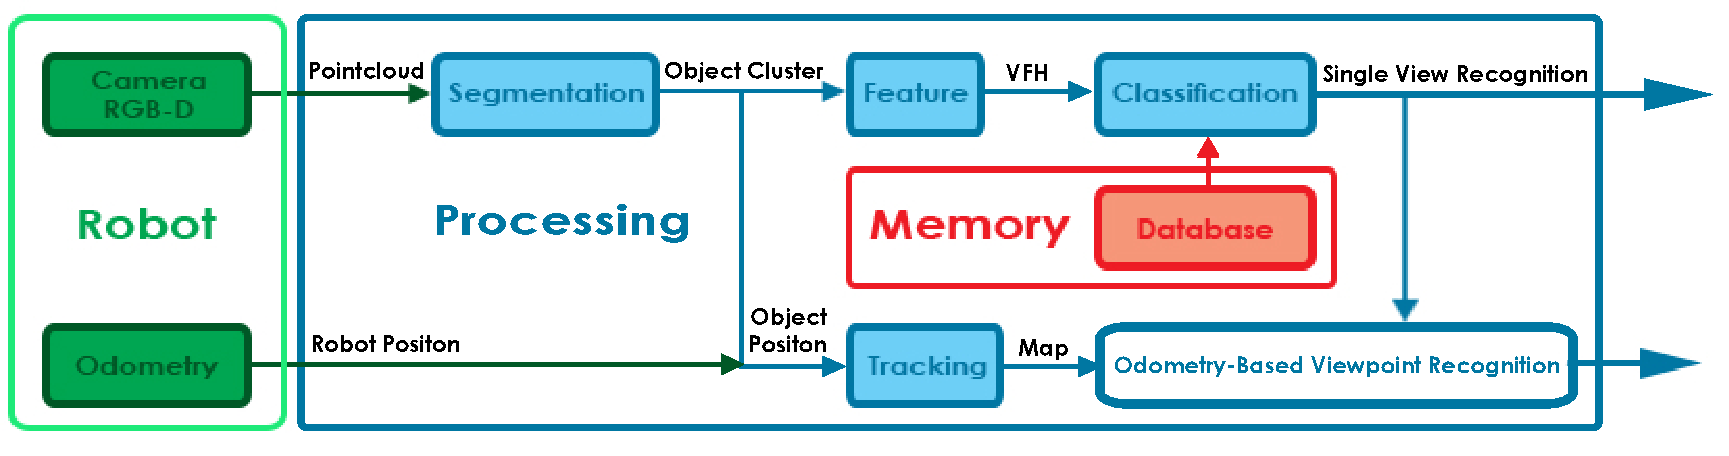
\includegraphics[width=15cm]{genarc.pdf}
  \caption{General achitecture of the system}
  \label{fig:architecture}
\end{figure*}

Precisely, the processing units takes as input the point cloud from the RGB-D sensor as well as the odometry measure. The first module consists in a segmentation stage that cleans up the point cloud by isolating objects of the scene into clusters of points. Those clusters are then sent to the feature extraction module to convert them to discriminative description histograms. Simultaneously, a cartography module converts the odometry data and the segmented object image position into the localization of scene elements in the world referential. Finally, the recognition module uses both the object feature and the evolution of those features compared to the displacement of the robot to retrieve the most likely object and view.

\subsection{Object Segmentation}

The segmentation algorithm used in this work is the one proposed by  Caron et al. \cite{caron2014neural}. The approach uses the same assumption that objects are lying on planes surfaces that can be found as the major plane of images. Furthermore, on our robot, the camera is always keeping the same orientation towards the floor. In this manner, its plan equation can be estimated once during a calibration step and used during the whole experiment. The segmentation algorithm uses the following steps

0) Calibration to obtain the floor plane equation before experiments, using RANSAC algoritm on an image where floor is the main plane.

 Then for each frame of the experiment:
\begin{enumerate}
\item Floor subtraction from the obtained equation
\item Points filtering if the distance to the sensor is more than 3 meters
\item Normal surfaces of the remaining points calculation
\item Filtering of big planes orthogonal to the ground. They are very likely to be walls
\item Projection of those points on the floor plane
\item Clustering of the projected points to create object candidates
\item Elimination of clusters that are too close to borders. They might not be objects, and their missing parts are likely to badly influence the recognition.
\item Centroid calculation of each remaining cluster (should be the objects of the image)
\end{enumerate}
Based on this algorithm, we obtain the position of each object in the camera frame, as well as the associated point cloud and normals.

\subsection{Object Representation}
The segmentation module provides a point cloud for each isolated object in the observed frame. This raw information is however not enough to efficiently discriminate the observed object and retrieve the associated view in the database. From the point cloud, we then extract two types of information. The first dimension of information relates to its position in the environment. This cartographic data allows the robot to track objects while moving around the scene, consequently, associating multiple views of it. A second dimension that can be translated in terms of visual and geometrical features is related to intrinsic characteristic of the objects capable of differentiating them from one another.

\subsubsection{Features} 
%Visual features used for the task of object recognition are either RGB-based or geometrical. Among RGB features, bag of words or SIFTs or color histograms are commonly used \cite{}. Deep features \cite{zhou2014learning} have also received a lot of attention recently, but their high dimensionality requires high computation performance to be processed in real time. Geometrical features based on point clouds are either local descriptor, such as SHOT \cite{tombari2010unique}, semi-global such as CVFH \cite{aldoma2011cad, aldoma2012our} descriptors or global \cite{rusu2009fast, rusu2010fast}. 

In our system, a global descriptor for each view is the easiest and best suited approach, as we need a way to efficiently compare a large number of view between a database and the current observation. We also restrict our descriptor to geometrical features that we found more discriminative than visual ones. 

Among global geometrical features, we selected the Viewpoint Feature Histogram \cite{rusu2010fast} - VFH. This feature captures in a single histogram the geometry of the object by estimating the angular transformation between the normal of each of its points and the standpoint from where it has been viewed. It is therefore discriminative of the object, but also the viewpoint at which it was observed. 

\subsubsection{Multi-view object representation}
\label{sec:aspectgraph}
% Change name
We define a multi-view representation based on polar aspect-graphs in order to store objects in the memory of the robot. This representation fuses both the intrinsic characteristics of the views of objects as well as the necessary movement to change between them.

\begin{figure}
 	\centering
	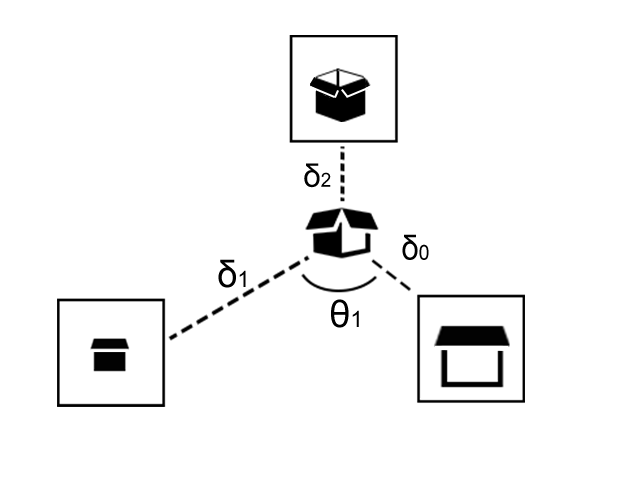
\includegraphics[width=0.3\textwidth]{object_model.png}
  	\caption{Multi-view object reprensentation based on a polar aspect graph}
	\label{fig:graphe_polaire}
\end{figure}

The polar referential is centered at the centroid of each object, illustrated in \ref{fig:graphe_polaire}. Its nodes represent the object aspect from a certain point of view, translated into a VFH histogram, and transitions from nodes are angular displacements obtained by the robot odometry. The use of VFH instead of viewpoint invariant features is then justified by this type of representation. Indeed, viewpoint information can bias the classification to search for eligible candidates in the database.


\subsection {Object Recognition based on multiple views and their relative positions}

Moving the robot around the environment produce a series of object observations. The idea behind our system is to find consistency between this sequence of possibly mis-recognized objects given a known displacement. In other words, tracking the positions of objects and the robot provides us an estimation of the physical transition between two successive viewpoints which can reinforce candidates as they are consistent with the movements prediction. To this end, we use a probabilistic model based on hidden Markov models.

\subsubsection{Viewpoint recognition based on a single observation}
\label{sec:singleviewpoint}

Regardless of odometry and cartographic data, a single observation provides a VFH histogram for each segmented object. Determining the  viewpoint of the object consists in finding the closest histogram in the database. To this end, the work from  Aldoma et al. \cite{Aldoma2012} suggest the use of a K-Nearest Neighbors, based on a chi-squared distance between histograms. The K-NN classifier has the great advantage of having both classification and training stages extremely fast for the intended database size. Thus, the closest viewpoint $V$ from the observation $O$ is retrieved based on the following equation:

\begin{equation}
\begin{cases}
  V = \underset{v_1 ...v_k} {\mathrm{argmin}} ~d(O,s_k)\\
  d(O, s_k) = \sum _i{ \frac{\left\|H_O(i)-H_{s_k}(i)\right\|^2}{H_O(i)}}
\end{cases}
\label{eq:chi-square}
\end{equation}

with $H_p(i)$ the $i$th bin of the VFH histogram of a point cloud $p$ and $s_1, ...s_k$ are the different views available in the database. Moreover, the distance $d(O,s_k)$ between an observation $O$ and a view $s_k$ in the database can easily be turned into a probability $P(O|s_k)$

\begin{equation}
\mathbf{P}(O|s_k) = \frac{d(O, s_k)}{d_{max}}
\label{eq:chi-prob}
\end{equation}
where $d_{max}$ is the maximum distance between two views of the database.

% Reading ...

\subsubsection{Object Tracking and Angular Displacement Estimation}

The segmentation algorithm provides us at each new frame a set of point clouds (one for each object) and associated centroid position in the camera sensor reference frame. On the other hand, we receive a signal of the speed of the wheels of the robot that we convert into a displacement estimation in the absolute reference frame. Therefore, we can convert both the position of the robot and point cloud centroids to the absolute reference frame. Nevertheless, imprecision from communication delays between processing modules, segmentation and object centroid calculation call for a filtering method to refine the absolute position of the observed objects. Moreover, because of the segmentation restrictions and constant displacement of the robots, objects are alternatively present and absent from the input image.

For that reason, we rely on a multi-tracker based on Kalman filtering that both refines the positions of each observed centroid and keeps an history of all observations and angular displacement for each tracked object from the beginning of the experiment. 

The multi-object tracker is composed with a set of Kalman filters, each of them tracking a single object and being updated as soon as a new observation of the object is found. Briefly, the update rule is done as follows: For each new frame, the centroid of all segmented objects are converted to the absolute reference frame. Then, their positions are compared with the position of the last observation of each available tracker (initially, no tracker is available). If the position of a centroid is close enough to the last observation of a tracker, the tracker is updated using Kalman update equations, and the pointcloud is added to the tracker history. If a centroid does not match with any Kalman position, the centroid is considered as a new object and a dedicated tracker is initialized.

This multi tracker relies on the two asumption that objects of the scene are static (although a dynamic model could be added) and that objects are separated of a minimum distance to avoid confusions between trackers.

Between two consecutive views $k-1$ and $k$ of the same object, an angular displacement is estimated to store the tracked object history with a polar aspect-graph representation (See section \ref{sec:aspectgraph}). The angular displacement is obtained by the following equation 

\begin{equation}
\delta_{k-1,k} = atan(p_{k-1} - p_{obj}) - atan( p_{k} - p_{obj})
\label{eq:triang}
\end{equation}
with $p_{k-1}$ and $p_{k}$ the absolute position of the robot for views $k-1$ and $k$, and $p_{obj}$ the absolute position of the centroid of the tracked object.


\subsubsection {HMM filtering}

Based on the sequence of observations and estimated angular displacement obtained with the odometry, we use Hidden Markov Models to retrieve the closest sequence of views in the database. This sequence not only provides us a reinforced recognition of the object, but also an estimate of the successive views at which the object was seen. The definition of our approach is inspired from \cite{le2014global}.

Given a track $T$ associated with $k$ observations ${O_1, ..., O_k}$ and $k-1$ angular transitions ${\delta_{1,2}, ..., \delta_{k-1,k}}$ between each of them, we model the viewpoint of the object from the robot sensor tracked by $T$ at time $k$ by a random variable $V_k$ that follows a Markovian process.

Based on the notations used in \cite{rabiner1989tutorial}, we define our HMM as $\lambda = \left\{N,M,\Pi,A,B\right\}$, with $N$ the number of states, $M$ the number of observations, $\Pi$ the initial state vector, $A$ the transition probability matrix, and $B$ the observation probability. 

In our case, a hidden state is associated with each viewpoints $s_i$, $0 < i \leq N$ in the database. $N$ is therefore the number of views in the database. As no prior assumption is made about the initial state of the system, we set $\Pi$ as a vector of length $N$ with equal probabilities.

The state transition probability matrix $A = \left\{a_{i,j}\right\}$ is defined as 

\begin{equation}
a_{i,j} = \mathbf{P}( V_k = s_i | V_{k-1} = s_j )
\label{eq:transmat1}
\end{equation}
or in other words, the probability of seeing view $s_i$ at observation $k$ given view $s_j$ at observation $k-1$. This probability  depends both on the angular displacement $\delta_{k-1,k}$ between the two observations, and the angular distances $\theta_{i,j}$ between views $s_i$ and $s_j$ in the database. Therefore, the transition probability is modified as each observation $k$ and defined as

\begin{equation}
    a_{i,j}^k =
   \begin{cases}
    1, & \text{if }  \theta_{i,j} < 2\delta_{k-1,k} \\
		\epsilon_1, & \text{otherwise}
\end{cases}
\label{eq:transmat}
\end{equation}
A small probability $\epsilon_1$ is attributed to unlikely transitions between the same object views to reinforce objects recognition rather than pose consistency. Transitions between views of different object are not allowed with zero probability of happening.

Last, the observation probability matrix $B = \left\{b_j\right\}$ is also constructed from each new observation. The distance from the K-NN is transformed in a probability distribution of the $K$ neighbors.

\begin{equation}
   b_{j}^k =  
   \begin{cases}
    \mathbf{P}(O_k|V_k=S_j), & \text{if }  s_j \in D_K \\
    \epsilon_2, & \text{otherwise}
\end{cases}
	\label{eq:emismat}
\end{equation}
where $D_K$ is the set of $K$ nearest neighbors and $\mathbf{P}(O_k|V_k=S_j)$ is the converted histogram distance into probability, defined by equation \ref{eq:chi-prob}. If the state view $S_j$ is not among the $K$ nearest neighbors, a small probability $\epsilon_2$ is associated instead.

Last, the Viterbi \cite{forney1973viterbi} algorithm is used to find the most likely sequence of views $\mathbf{V}$ given the HMM $\lambda$, and the sequence of observations $\mathbf{O} = \left\{O_1, ... O_M\right\}$. 
\begin{equation}
\mathbf{V} = \underset{\mathbf{S}} {\mathrm{argmax}} ~\mathbf{P}(\mathbf{S}|\mathbf{O}, \lambda)
\label{eq:viterbi1}
\end{equation}

The Viterbi path of the track with observations $\mathbf{O}$ then coincides with the sequence $\mathbf{V}$ of recognized view from $\mathbf{O}$. The optimization is solved using the following equations

\begin{equation}
  \begin{array}{rcl}
    V_{1,i} &=& b_k^1 \cdot \pi_i \\
    V_{k,i} &=& \underset{j \in \left\{1, ... N\right\}} {\mathrm{max}} \left( b_k^i \cdot a_{j,i}^k \cdot V_{k-1,j}\right)
  \end{array}
	\label{eq:viterbi}
\end{equation}
where $\pi_i$ is the probability of initially being in $i$th state (from $\Pi$ vector), and $V_{k,i}$ is the probability that the most probable sequence based on the $k$ first observations ends up in state $s_i$. The most probable sequence is then retrieved by taking the sequence of $V$ of successive states used to compute $V_{M,i}$ so that
\begin{equation}
  \begin{array}{rcl}
    s_i &=&\underset{s_j, j \in \left\{1, ... N\right\}} {\mathrm{Argmax}}(V_{M,j})
  \end{array}
\end{equation}


\section{Experimental results}
The proposed recognition system was deployed in a differential mobile robot, the Wifibot V2, embedded with a RGB-D camera, Asus Xtion Pro Live. The algorithm architecture was implemented over ROS using PCL and OpenNi2 libraries. 

In order to validate the approach, the robot was initially taught aspects graphs from chosen objects and two sets of experiments were proposed to analyze the efficiency of the algorithm in realistic scenarios.

 
%In order to succeed, the robot must face inexistent viewpoints due to a sparse database, blurred images from motion and object spatial symmetry

\subsection{Object Database}
First, twenty objects varying in size and shape (monitor, boxes, chairs, trashcans, people, ...) were selected to compose the knowledge database of the robot. The aspect graphs of each object were obtained with VFH features from \textit{eight} equally distant viewpoints acquired from positioning the robot around the to be learned object 1.5 meters away. This way, the angular position between two consecutive views was easily and accurately determined and stored.  % Each of the feature was labeled with its polar coordinate using 

%For each of them we moved the robot to make a complete circle around them separately. Eights view were obtained from each circle, so that the angular distance between each of them was 45 degrees. The point cloud and associated features were extracted and recorded for each view.
 
\subsection{Odometry Contribution}
% Le mal fonctionnement du tracking a fait qu'on a des arcs de cercle au tour des objects qui commencent de positions al�atoires. Dans le cas o� le tracking a march� on a seulement quatre cercles complets
The first experiment consist in a comparison between the performance in recognition between single-view and multi-view recognition techniques. In other words, this comparison attest whether the proposed architecture is interesting or not, since having the same or worst performance by the cost of adding a complex post-processing and tracking modules is not interesting.

Technically, each object was partially circled by the robot from at least four random initial positions at speed of $0.35 \pm 0.1 m/s$. The robot recorded for each run between 5 and 30 frames at different viewpoints of the object, and tried to recognize them using both recognition algorithms.

A typical experiment is illustrated in Figure \ref{fig:resultats_expe}. The first row represents the image sequence segmented by the robot for a given object at each new frame. This is the object to be recognized. The second line, is the viewpoint recognition based on a single image, without using any odometric information. The only measure used to recognize the view is provided by the distance to the nearest neighbor in the database (see section \ref{sec:singleviewpoint}). Interesting is to notice that the rotation invariance of the VFH descriptor actually tricks the view estimation by taking the symmetrical correspondent in the first red square. In addition, the back of the penguin is a large and almost flat surface. It is, therefore, considered as background wall by the segmentation module and almost entirely removed. The resulting point cloud is insufficient to accurately characterize the view, thus leading to wrong view detection in the blue squares. The last row represent the final output of the Viterbi algorithm. As expected, the combination of VFH-based view estimation and odometry is able to retrieve the correct sequence of views.

\begin{figure*}
	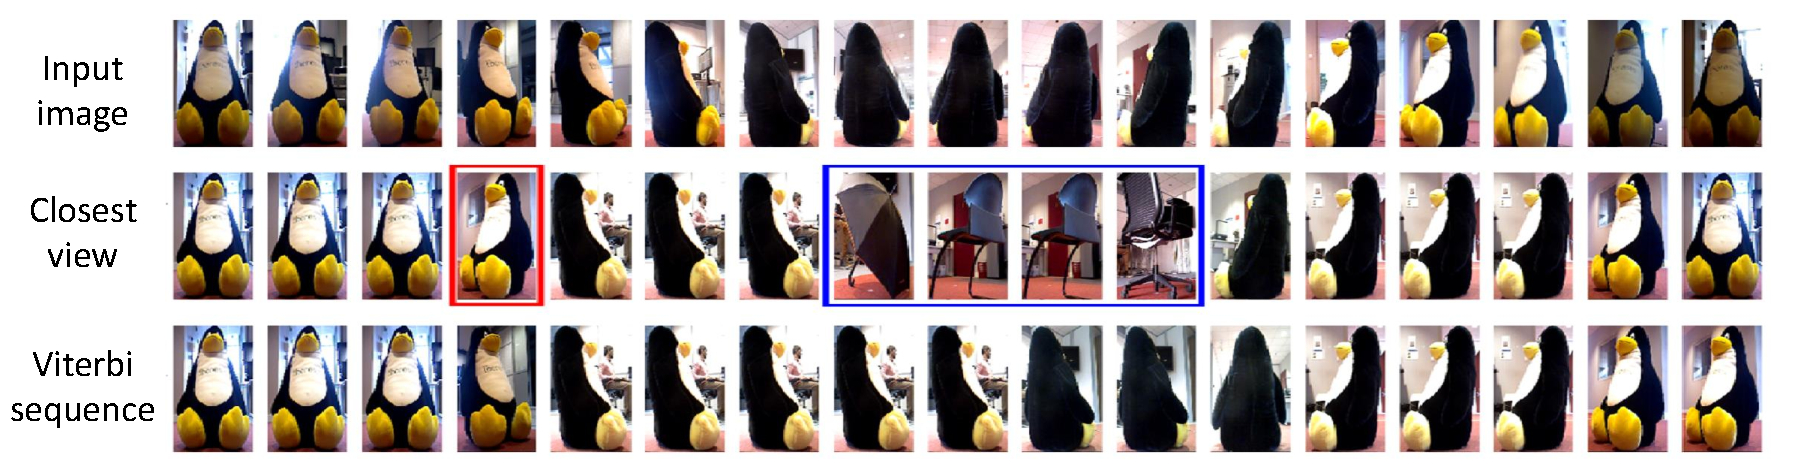
\includegraphics[height=4.7cm]{hmmexample.pdf}
			\caption{\textbf{Typical experiment} - The HMM refinement makes self correction of irrelevant views estimation, even when objects were badly segmented during the database creation.}
	\label{fig:resultats_expe}
\end{figure*}

The experiment was then numerically evaluated by comparing the performance of the two approaches as the number of views was increased, displayed in Figure \ref{fig:comp}. Dashed curves represent object and view recognition on a single image basis. Solid ones are obtained based on multi-view estimation. When the number of observation is low, the mono-view recognition tends to be slightly better than multi-view. The gap between mono and multi-view recognition increases with the number of observations. With 25 or more observations, the multi-view  recognition outperforms the mono-view by 30\% for object recognition and 40\% for view estimation. Last to make sure that odometry has an impact in the object recognition process, we compare the results obtained from the Viterbi sequence ('\textit{multi+odom obj}') with the recognition rate when using only the average probabilities provided by equation \ref{eq:chi-prob} over the sequence ('\textit{multi obj}'). In this case, the recognition rate gap is around 7\%.

\begin{figure}
	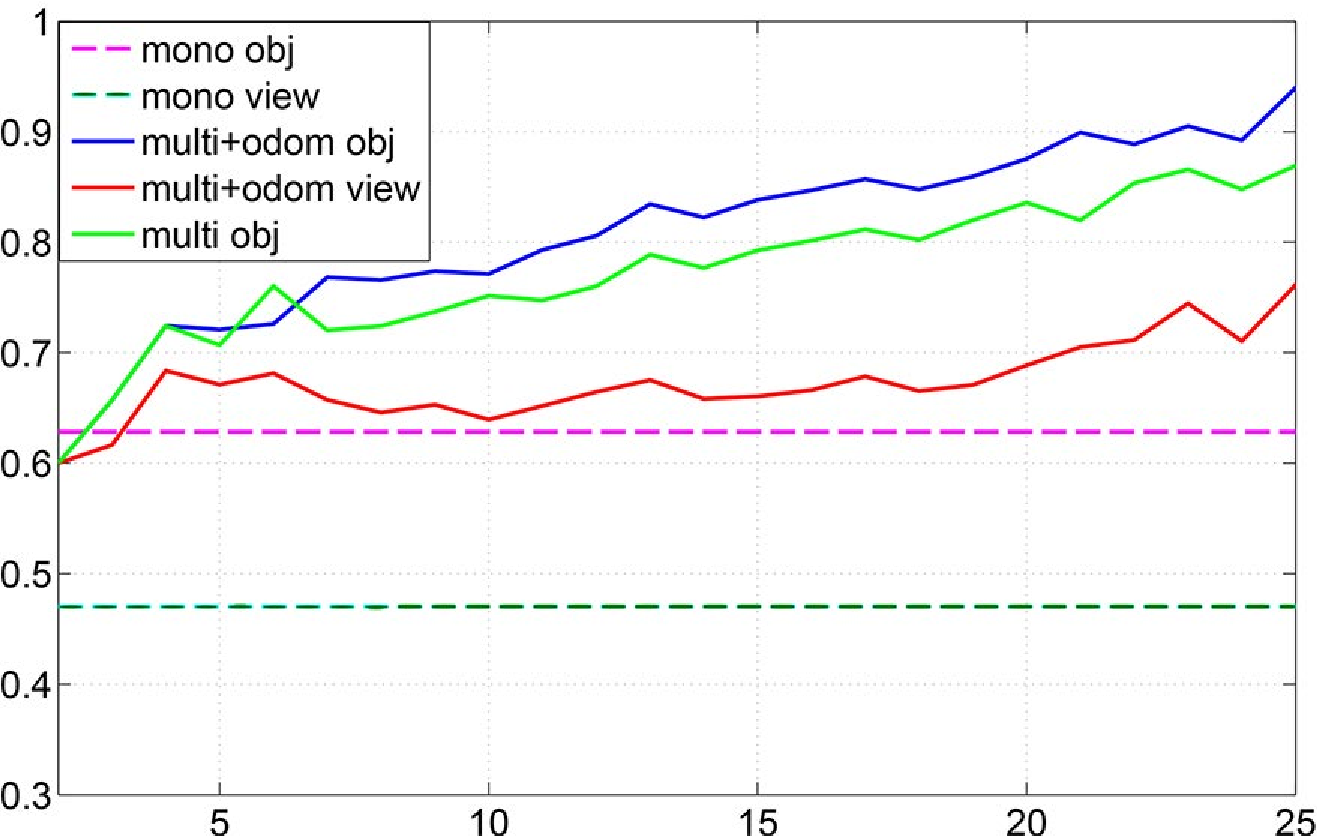
\includegraphics[width=8.65cm]{recog_plot.pdf}
	
	\caption{\textbf{Numerical results evaluation} - Evolution of the correct recognition rate versus the number of views. Both for objects and view recognition, the multi-view approach outperforms the mono-view approach.}		
	\label{fig:comp}
\end{figure}

\subsection{Multi-object recognition}
In a second evaluation, concurrently with the recognition efficiency, the multi-tracking capabilities were put into test. Tracking objects correctly has a critical impact on the overall performance of the system.

The experiment consists in moving the robot around a room full of objects, making sure to visualize them from different perspectives. A typical view from the robot as well as associated segmentation result is presented in Figure \ref{fig:mono_recon}. This scenario is a much more complex case than the first one as moving in a room with many elements generates occlusions, thus leading to incomplete point clouds and biased feature descriptors. An simple evaluation of the multi tracking is displayed in Figure \ref{fig:multi_map}. Thee possible scenarios can leard to tracking failure. First, the object is never segmented and no track is open for it. Second, more than one track are opened for the same object. This may happen if an object is segmented in two different clusters or it is not seen for a long time and its estimated position error is too high . Third, two objects are merged in the same track. This may happen if objects are too close from each other. In the case of Figure \ref{fig:multi_map}, the object 'Chair4W' has two tracks for the same object. On the other hand, Figure \ref{fig:recon} provides another sequence example on which two different tracks were fused. In this case, the person and the fan were too close from each other, and a track mixing both entries was created. The result is the identification of the 'fan' in a track that is mainly composed with 'person' observations.

\begin{figure}
	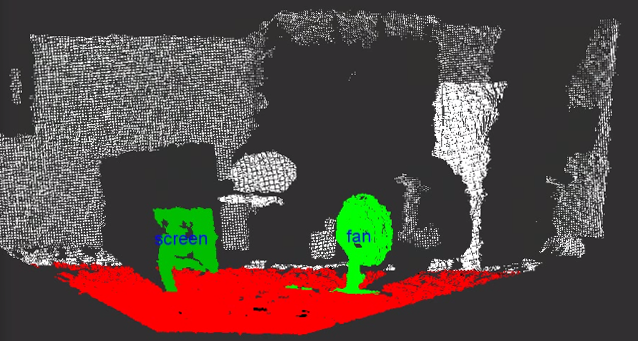
\includegraphics[width=8.65cm]{mono_recon.png}
	\caption{\textbf{Result of object segmentation and identification} The red points represent the floor plane and the ignored white ones exceed the three meters threshold. One could also notice the infra-red shadows created by objects, potentially leading to occlusions}
	\label{fig:mono_recon}   
\end{figure}

\begin{figure}
	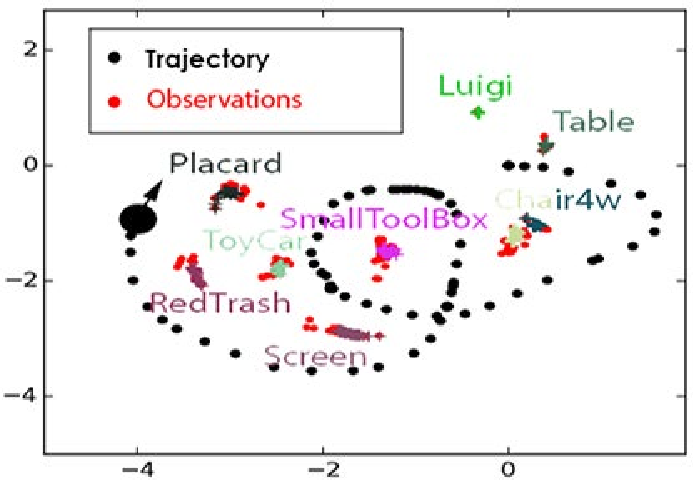
\includegraphics[width=8.65cm]{map.pdf}
	\caption{\textbf{Mutli-objects tracking results} - Red dots corresponds to segmented objects centroids. Each color cross stands for the position estimation from a tracker. Each filter is associated with a unique color. Theoretically, a single filter should be associated with a single object. Black dots represent the trajectory of the robot during the experiment.}	
	\label{fig:multi_map}
\end{figure}


In the sequence presented in Figure \ref{fig:recon}, Four of the five objects present in the scene were correctly recognized. As explained earlier, the only object recognition mistake is because the first object, a person, was too close to the fan and were considered as one single object by the tracker.


\begin{figure}
	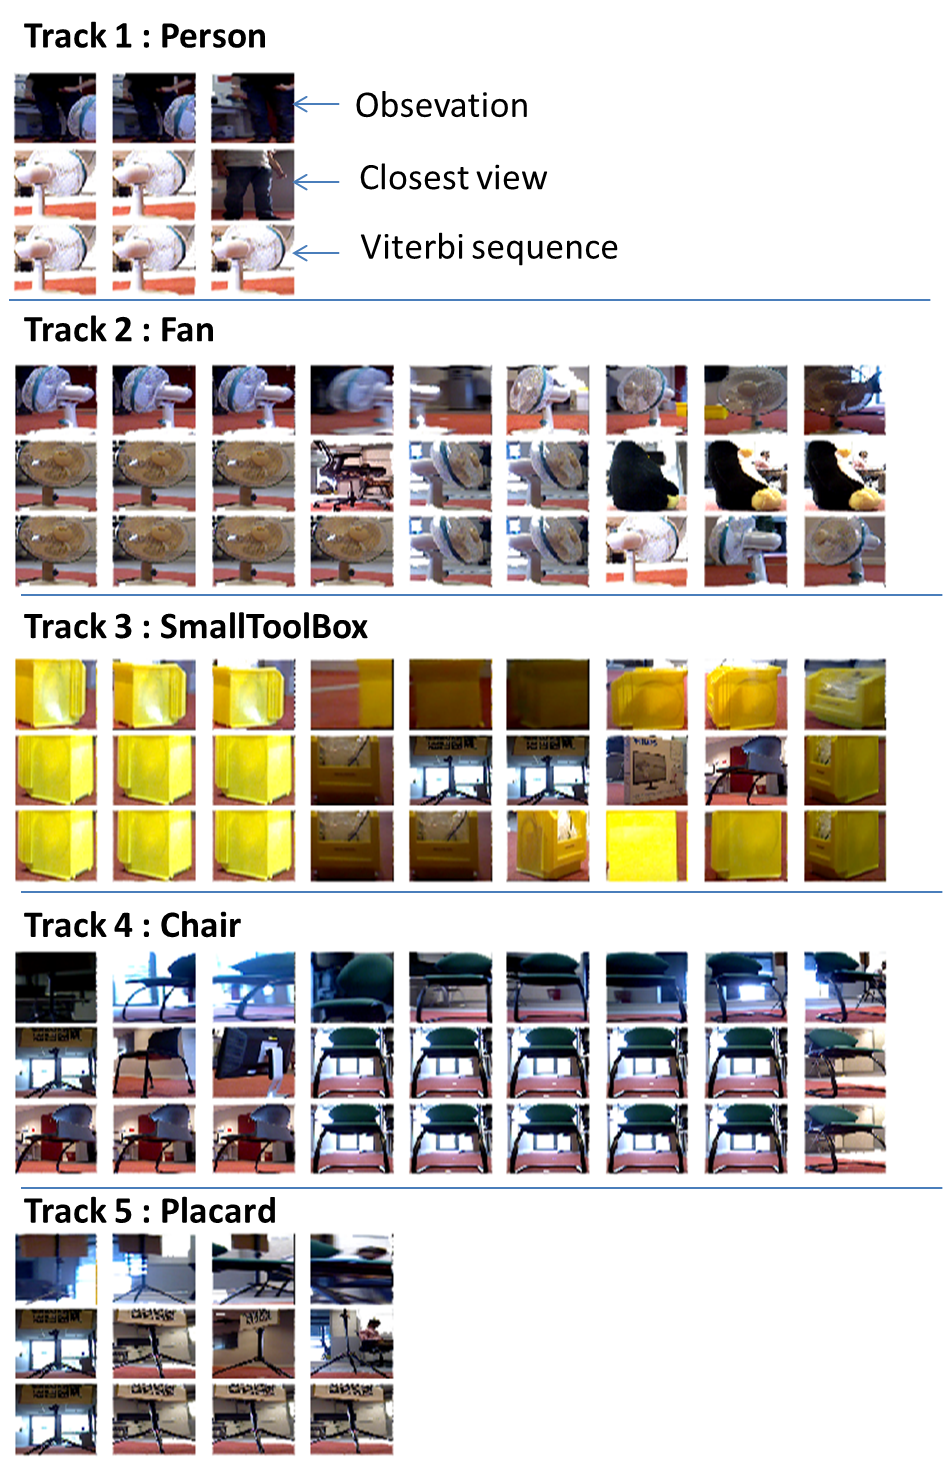
\includegraphics[width=9cm]{multi_recon3.png}
	\caption{\textbf{Example of multi-view recognition in a scene with five objects.}}
	\label{fig:recon}
\end{figure}

\section{Conclusion}

The proposed method focuses on integrating odometry information to boost recognition efficiency, based on the intuition that different perspectives of the object and analysis of transitions between them provides unexplored information. The results from practical experiments shows that the odometry-based algorithm outperforms the classical one in both object and viewpoint recognition, strengthening the interest in a more sophisticated pipeline. Moreover, the approach has the advantage of not being platform specific, which means it could be implemented in any mobile system equipped with a RGB-D sensor and capable of measuring its position.  However, the algorithm is quite sensitive to bad segmentation, specially if a object is divided into two disjoint clusters. Errors due to occlusion could be reduced using semi-global descriptors and a more exigent segmentation. 

Future work will consist in recognizing moving objects, where the recognition feeds the tracking module with the moving dynamics of the target, and including object transformation by allowing state transitions to views of other objects \footnote{i.e. human moving towards a chair and sitting down, creating a new object human+chair}. A more immediate challenge is to create the object database on the fly once a new observation is not encountered on it, according to a distance threshold.

%A relatively general object model capable of representing a huge variety of everyday objects. 


\bibliographystyle{plain}
\bibliography{rapport}
\end{document}
